In a dense target environment, the gating technique is not sufficient enough to discriminate between detections. Thus a further assignment logic has to be implemented. Conflicts can occur for instance, when a detection satisfies the gating of different tracks, or when a track was multiple detections within its gate. This problem is called the assignment problem. 

There are basically two types of solutions. The  \ac{nn}-approach (\cref{mtt:nn}) and the "all-neighbors" approach (\cref{mtt:pda} and \cref{mtt:jpda}). The first step of all solutions, however, is the same. First, an assignment matrix is built. For this, the norm of the innovation vector that would result if track $i$ and detection $j$ would be assigned is defined as 

\begin{equation}
d_{ij}^2 \triangleq \vec{v}_{ij}(n)^T \matrix{S}_i^{-1}(n)\vec{v}_{ij}(n)\\,
\end{equation}
where $\matrix{S}_i(n)$ is the residual covariance matrix defined in \cref{eq:innov}. Furthermore, it is assumed that the residual has a Gaussian distribution
\begin{equation}
	g_{ij} =\frac{\exp(-\frac{d_{ij}^2}{2})}{(2\pi)^{M/2}\sqrt{|\matrix{S}_i|}}\\,
\end{equation}
where $M$ is the measurement dimension and $|\matrix{S}_i|$ the determinant of $\matrix{S}_i$.
\begin{figure}[h]
	\centering
	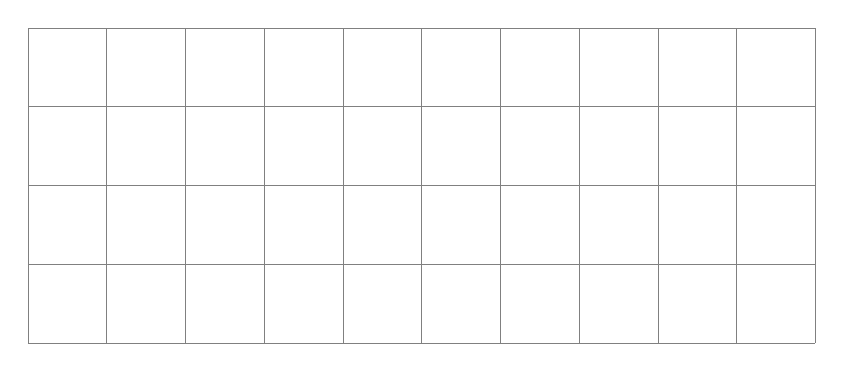
\begin{tikzpicture}
% Reference Grid
\draw[gray,very thin] (0,0) grid (10,4); 

\end{tikzpicture}
	\caption{Example of conflict situations for assignment}
	\label{fig:assign}
\end{figure} 

The basic goal is to make assignment decisions based on the maximization of $g_{ij}$, which is equivalent to minimizing the quantity 
\begin{equation}
	d_{Gij}^2 = d_{ij}^2 + \ln |\matrix{S}_i|\\,
\end{equation}
which will be used as distance function for use in the assignment problem.

